\chapter{Placement}
\label{chap:Placement}

\section{Introduction}
\label{sec:Placement-Introduction}
Les systèmes-sur-puce modernes contiennent tant des circuits numériques que des circuits analogiques. La conception de circuits numériques a été particulièrement automatisée par des outils de conception assistée par ordinateur tandis que la conception de circuits analogiques est restée manuelle. Avec l'évolution des nouvelles technologies nanométriques, cela implique un travail manuel long et sujet à l'erreur humaine. \newline 

\indent Dans le cadre des circuits analogiques, les parasites du dessin des masques et les contraintes de procédés de fabrication augmentent drastiquement la complexité de la tâche quant au placement des modules du circuit. Il devient essentiel d'introduire des outils de placement dédiés aux circuits analogiques dans le but d'accélérer aussi bien le cycle de conception que l'effort de conception. \newline 

\indent La phase de placement pour les circuits mixtes et analogiques a une influence importante sur les performance du circuit. La relation de placement entre l'ensemble des modules, et plus particulièrement celle entre les modules appariés, est importante afin de préserver au plus possible l'environnement adéquate de fonctionnement des modules en tenant compte des parasites engendrés par le dessin des masques. \newline

\indent Dans ce chapitre, nous discuterons de l'étude du problème du placement des circuits mixtes et analogiques. \newline

\indent Dans la section \ref{sec:Placement-SoA-topologie}, nous énumérons les principales représentations topologiques du plan de masse de l'état de l'art. Ces représentations utilisent des graphe traduisant des relations de placement entre l'ensemble des modules d'un circuit. Leur spécificité avec leurs avantages et inconvénients et les contraintes qu'elles sont capables de prendre en compte dans le choix d'un placement optimal seront explicités. \newline 

\indent Dans la section \ref{sec:Placement-SoA-optimization}, nous exposerons la phase d'optimisation que la majorité de l'état de l'art utilise dans le cadre de la recherche d'une solution de placement optimale. Les algorithmes de recuit simulé ont souvent opté pour leur capacité à produire de bons résultats en temps suffisamment court. Ces algorithmes sont également relativement simples à implémenter et peuvent être facilement enrichis pour des conditions supplémentaires. \newline

\indent Dans la section \ref{sec:Placement-Implémentation}, nous présenterons notre approche du problème du placement des circuits mixtes et analogiques. Notre représentation topologique ainsi que notre méthodologie d'optimisation y sera détaillées. Cette section contiendra une partie de notre structure de données utilisée tout au long de la génération du placement routage. \newline

\indent Dans la section \ref{sec:Placement-Exemple}, les détails de la méthodologie de placement seront illustrés par un exemple contenant des contraintes de placement répandues. Les interventions du concepteur seront énumérés avec clarté dans le but de mettre en avant son rôle dans le choix de la solution de placement.

\section{\'Etat de l'art des algorithmes de placement}
\label{sec:Placement-SoA}

\indent Le problème de placement abordé par les outils de CAO dédiés aux dessins des masques numériques et analogiques consistent à explorer un grand espace de solutions de configurations de placement faisables et non faisables en utilisant une représentation du plan de masse couplée à une optimisation stochastique telle que l'algorithme de recuit simulé. A la différence des circuits numériques, les circuits analogiques doivent prendre en considération des contraintes de placement supplémentaires liées aux parasites du dessin des masques. L'état de l'art des approches de placement pour circuits mixtes et analogiques sera abordé dans les sections suivantes. 
\subsection{Les représentations topologiques de plan de masse}
\label{sec:Placement-SoA-topologie}

Afin de pouvoir générer un placement légal respectant plusieurs contraintes de placement analogiques, la majorité des études récentes emploie une représentation sous forme de graphe. On distigune deux catégories de représentations: les représentations absolues et les représentations topologiques. Les représentations absolues \cite{Jepsen83} sont principalement dans les anciennes méthodes de placement et consiste à associer à chacun des modules du circuit une coordonnée par rapport à un point de référence. Cette représentation permet la superposition illégale de modules lors de la phase d'optimisation dû au fait qu'il n'existe pas de relation de placement entre les modules. Cette approche doit alors être en mesure explorer un très grand espace de solutions comprenant tant des placements faisables que non faisables. Cela se traduit par des temps d'exécution long causés par le grand nombre de mouvements nécessaires pour obtenir un dessin des masques satisfaisant. Il est également possible qu'en plus du long temps d'exécution, il ne garantie pas toujours de solutions faisables. L'ajustement de la fonction de coût pour éviter les recouvrements de modules peut requérir un effort conséquent. \newline

En opposition aux représentations absolues, les représentations topologiques ne font pas face à des problèmes de recouvrements, elles consistent à définir des relations de positions entre les modules d'un circuit. Ces représentations sont largement utilisés pour des raisons d'efficacité et de flexibilités à pouvoir satisfaire des contraintes pour un moindre coût en termes de nombre de mouvements comparées aux représentations absolues. On présentera dans les sous-sections suivantes les représentations topologiques les plus utilisées de l'état de l'art. 
\subsubsection{Les slicing models}
Les {\it slicing models} \cite{Wong1986} font parties des premières représentations topologiques utilisées. Ces {\it slicing models} sont représentés à l'aide d'un graphe appelé {\it slicing tree}. Un {\it slicing tree} est un arbre dans lequel chaque noeud interne peut être obtenu par découpes récursives du circuit (Fig. \ref{fig:1}). A partir de la région totale du circuit représentant la racine de l'arbre, le circuit sera découpé de manière hiérarchique, alternativement de manière horizontal et vertical, jusqu'à atteindre les feuilles de l'arbre représentant les modules du circuit ou bien des espaces de routage. L'ensemble des rectangles terminaux dû aux découpes sera toujours représenté par une feuille. \newline
\begin{figure}[h]
\begin{center}
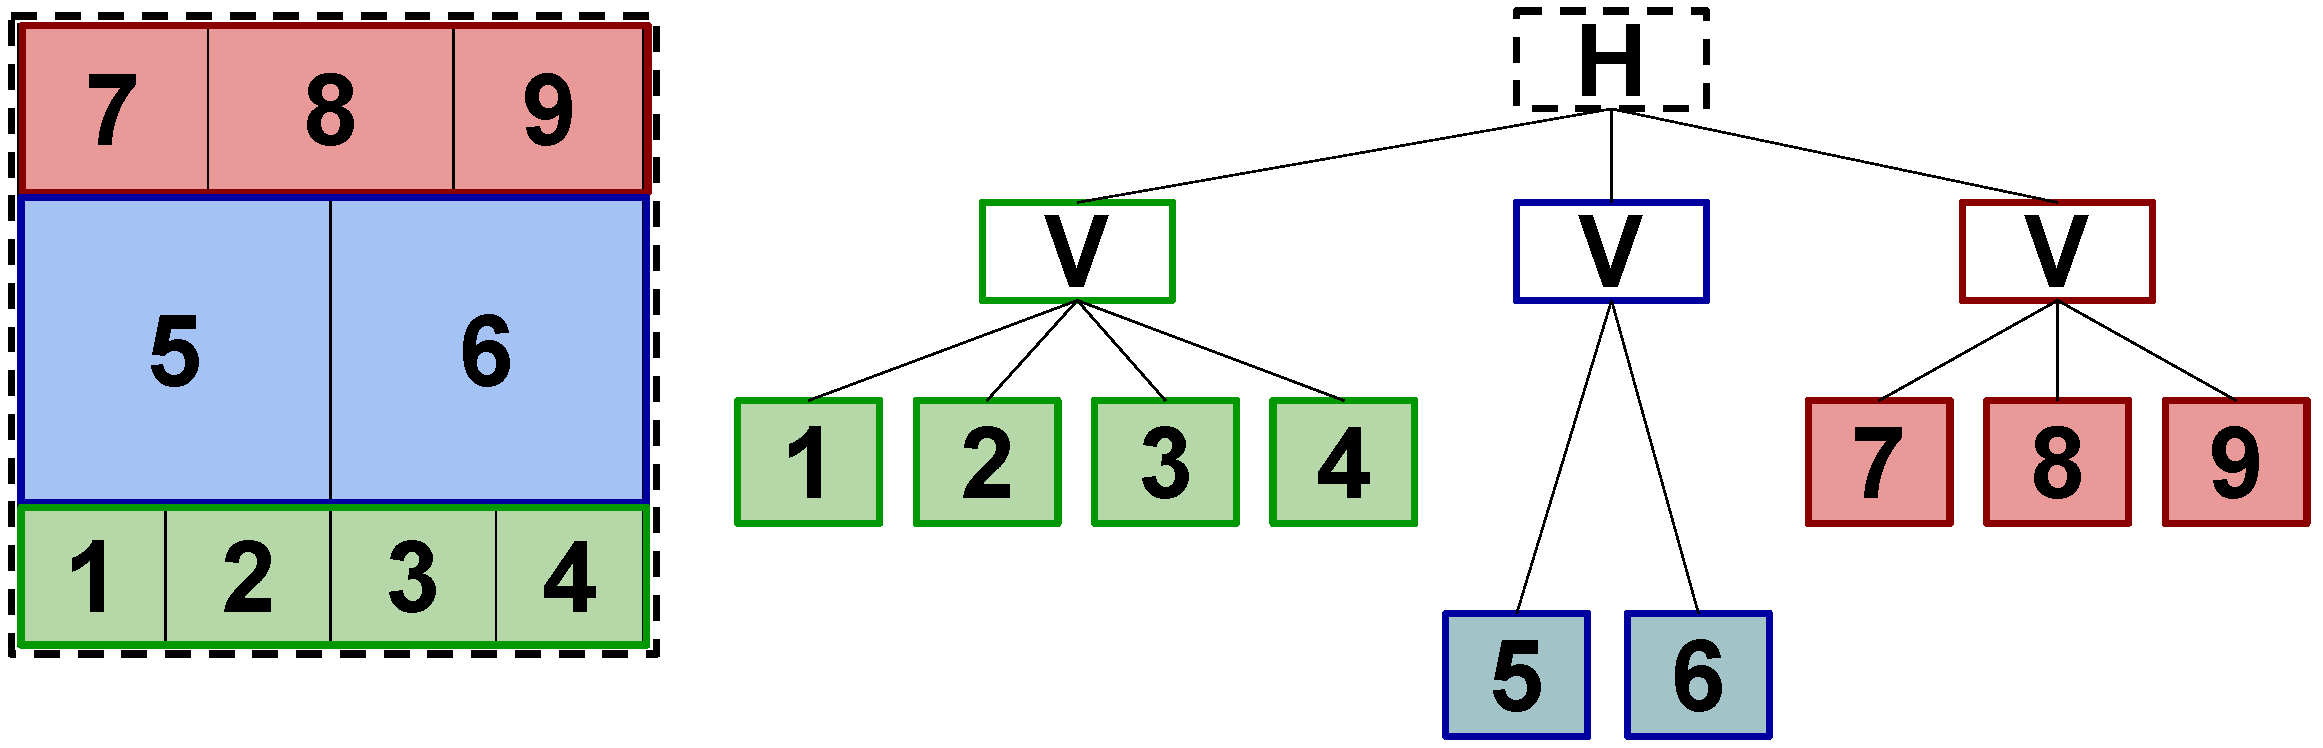
\includegraphics[height=0.17\textheight]{Figures/1.pdf}
\caption{Exemple de placement et sa représentation en {\it slicing tree} ou "H" définit une coupe horizontal et "V" une coupe vertical.} 
\label{fig:1}
\end{center}
\end{figure}  \newline
\cite{Abthoff1996} concentre son optimisation sur la surface totale du circuit ainsi que la longueur total des {\it nets} dont l'amélioration est 5 fois plus courte comparé à la non prise en considération. L'optimisation prend en compte les contraintes de proximité, de modules pré-placés et de symmetries. \cite{Prieto1997} considère les parasites d'interconnection dans la phase d'optimisation avec une prise en compte simultanée du placement et routage. Ils sont en mesure de maintenir des symmetries de groupes de modules. \cite{Young1998} étend l'approche de \cite{Wong1986} afin de pouvoir considérer des modules pré-placés, de contraintes de bordure \cite{Young1999} et de proximité \cite{Young2000}. \cite{lina2012} améliore la formulation des {\it slicing trees} en introduisant des conditions de symmétries pour des groupes de modules. \cite{Wu2012} introduit la prise en compte des contraintes de sens du courant dans les structures en {\it slicing tree} en plus des symétries. \newline

Puisque tous les circuits n'ont pas une structure en tranche, le désavantage de cette topologie est que la densité de la solution de placement peut être dégradé ce qui peut être notable lorsque les modules d'un circuit ont des rapports hauteur/largeur très hétérogènes. De plus, la structure des {\it slicing trees} ne permet pas de représenter toutes les placement possibles (Fig. \ref{fig:2}). Suite à ces limitations, des représentations avec des structures {\it non-slicing} se sont succédé. Les {\it sequence pairs}, les {\it B*-trees}, les {\it Ordered-Trees - O-tree} et les {\it Transitive Closure Graphs - TCG} seront présentés dans les sous-sections suivantes.
\begin{figure}[h]
\begin{center}
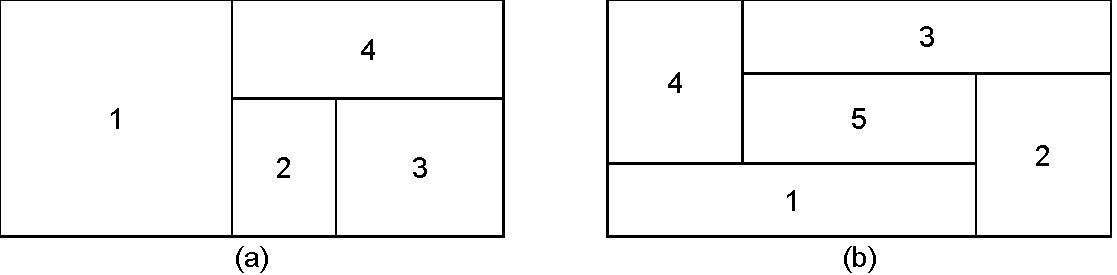
\includegraphics[height=0.15\textheight]{Figures/2.pdf}
\caption{Exemple d'un placement représentable par un {\it slicing tree} (a) et d'un placement non représentable (b)} 
\label{fig:2}
\end{center}
\end{figure}
\subsubsection{Les sequence pair}
Les {\it sequence pairs} sont utilisés dans le context des placements de circuits analogiques pour la première fois par \cite{Balasa2000}. Une {\it sequence pair} donnée pour ensemble de modules est une paire de séquences contenant l'ensemble des modules. Par example, $(abc, cba)$ est une {\it sequence pair} pour l'ensemble de module \{$a,b,c$\}. Pour un placement donné, la sequence pair correspondante est obtenue par la construction des échelons positifs et négatifs de chacun des modules (Fig. \ref{fig:3}). L'échelon positif (négatif) d'un module contient 3 parties: l'échelon haut-droit (gauche-haut), l'échelon bas-gauche (droite-bas) et la ligne diagonale effectuant la connexion. L'échelon  haut-droite (bas-gauche, gauche-haut, droite-bas respectivement) d'un module est $A$ est dessiné en suivant les règles suivantes:

\begin{enumerate}
\item On part de coin supérieur droit (inférieur gauche, supérieur gauche et inférieur droit respectivement) du module $A$.
\item On change la direction alternativement haut (bas, gauche et droite respectivement) et droit (gauche, haut et bas respectivement) jusqu'à atteindre le coin supérieur droit (inférieur gauche, supérieur gauche et inférieur droit respectivement) du placement sans croiser:
\begin{itemize}
\item Les bordures des autres modules
\item Les lignes précédemment tracées
\end{itemize}
\end{enumerate}
En utilisant l'ordre des séquences des échelons positifs et négatifs (de la gauche vers la droite), une paire ordonnée, ($\Gamma_+, \Gamma_-$), de séquences de modules peut être placé. La Fig. \ref{fig:3} montre le placement résultant de ses échelons négatifs et positifs avec de ses séquences respectives. A partir d'une {\it sequence pair}, il est également possible d'en dégager les contraintes géométriques (horizontal ou vertical) entre deux modules.

\begin{figure}[h]
\begin{center}
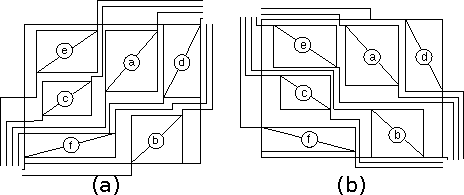
\includegraphics[height=0.22\textheight]{Figures/3.pdf}
\caption{(a) \'Echelons positifs résultant et $\Gamma_+=ecadfb$. (b) \'Echelons négatifs résultant et $\Gamma_-=fcbead$.} 
\label{fig:3}
\end{center}
\end{figure}

H. Murata et al. \cite{Murata1996} sont les premiers à introduire le concept de {\it sequence pair} pour des applications de dessins des masques {\it VLSI} durant une période pendant laquelle les {\it slicing models} étaient populaires mais ne produisaient pas des résultats assez satisfaisant. \cite{Balasa2000} adresse l'utilisation des {\it sequence pairs} dans le cadre du placement pour circuits analogiques avec une prise en compte de contraintes de symmétries et \cite{Balasa2001} améliore leur temps de calcul par la suite. \cite{Cheong2006} ajoute la considération d'alignement et de contraintes de proximités des modules en plus des symmétries. \cite{Long2006} oriente leur attention sur du placement vis à vis du sens du courant tout en tenant compte des symétries. \cite{Nakatake2010} porte leur attention sur les contraintes de regularités couplés aux contraintes de symmétries. \cite{Xiao10} prends en considération des contraintes de congestions pour le routage en évaluant la congestion des placements donnés. 

\subsubsection{Les O-trees}
\begin{figure}[h]
\begin{center}
  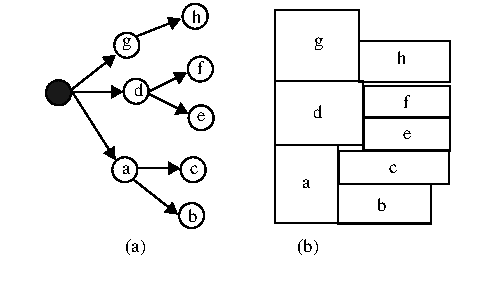
\includegraphics[height=0.24\textheight]{Figures/5.pdf}
  \caption{(a) Une représentation en {\it O-tree} et (b) son placement correspondant.}
\label{fig:5}
\end{center}
\end{figure}
Un ({\it Ordered Tree (O-tree)}) étend le principe des {\it B*-tree}  à une représentation du plan de masse de type {\it non-slicing} avec une complexité inférieur à celle des {\it slicing models}. \'Etant donné un placement de $n$ modules, un {\it O-tree} correspondant possède $n+1$ noeuds encodé par ($T,\pi$), o\`u $T$ correspond à une chaine de caractères de 2$n$-bit identifiant la structure de l'arbre et $\pi$ représente l'ordre des noms des modules sans considérer la racine de l'arbre. Lorsqu'on parcourt l'arbre en profondeur, "0" correspondant à une arête descendante, et "1" à une arête ascendante. Cette méthode permet de réduire les redondances et le temps d'exécution est plus rapide que celui des représentations en {\it sequence pair}. \newline

Cette méthodologie est introduite par \cite{Guo1999}, \cite{FlorinBalasa2000} et \cite{LinfuXiao2009} élargies les types contraintes de symétries considérées.

\subsubsection{Les B*-trees et HB*-trees}
\begin{figure}[h]
\begin{center}
  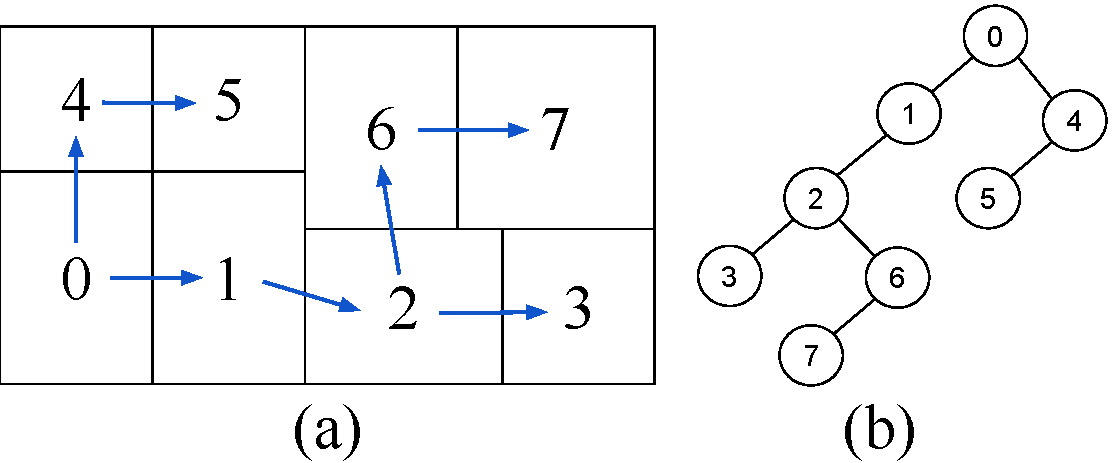
\includegraphics[height=0.19\textheight]{Figures/4a.pdf}
  \caption{(a) Placement compact. (b) Représentation en {\it B*-tree} du placement compact (a).}
\label{fig:4a}
\end{center}
\end{figure}
 Les ({\it Ordered Binary Trees - B*-trees}) sont des arbres couramment utilisés pour représenter un placement compacte de modules dans lequel tous les modules ne peuvent plus se déplacer vers la gauche et vers le bas. Chaque module d'un circuit est représenté par un noeud dans un {\it B*-tree}. La racine d'un {\it B*-tree} correspond au module situé dans le coin inférieur gauche, il s'agit du module 0 sur la Fig. \ref{fig:4a}. Le noeud de gauche du module 0 représente le module de droite et adjacent au module 0, il s'agit du module 1. Le noeud de droite du module 1 représente le module au dessus et adjacent au module 0, il s'agit du module 4. La Fig. \ref{fig:4a} montre un placement et sa représentation en {\it B*-tree} correspondante. \newline

Les {\it B*-trees} sont introduits par \cite{Balasa2000.2} et \cite{Chang2000} dans le but d'utiliser une réprésentation succédant aux {\it O-trees}. Cette approche est amélioré en incorporant les contraintes de symmétrie par \cite{Balasa2002} dans le cadre des circuits analogiques. \cite{Maruvada2005} améliore le temps d'execution de 20\% à 30\%. \cite{Strasser08} propose une approche déterministe permettant une meilleure reproductabilité du placement. \newline

La représentation des B* avec s'enrichie avec l'utilisation des {\it Hierarchical Ordered Binary Trees - HB*-trees} \cite{Lin09} dans le but d'ajouter des contraintes hierarchies et groupes de symétries. \cite{Lin2010} y ajoute la prise en compte de contraintes de bordure. Cette représentation est ensuite utilisé pour différentes contraintes d'optimisation, telle que pour des contraintes de température \cite{Lin11} ou de régularité \cite{Chou2011} et avec de meilleur optimisation de temps d'execution \cite{Tsao2011}.

\subsubsection{Les Transitive Closure Graph}
Les {\it Transitive Closure Graphs (TCG)} décrivent les relations géométriques entre les modules d'un circuit en se basant sur deux graphes: un {\it Horizontal transitive closure graph $G_h$} et un {\it Vertical transitive closure graph $G_v$}. Dans le {\it $G_h$} (respectivement {\it $G_v$}), une arête $<v_i,v_j>$ exprimé que le module $m_i$ se trouve à gauche de (respectivement en bas de) la cellule $m_j$. Le poid associé à l'arête dans {\it $G_h$} (respectivement {\it $G_v$}) correspond à la largeur (respectivement hauteur) du module associé. La Fig. \ref{fig:6} montre un example de placement avec sa représentation {\it TCG}. \newline

\begin{figure}[h]
\begin{center}
  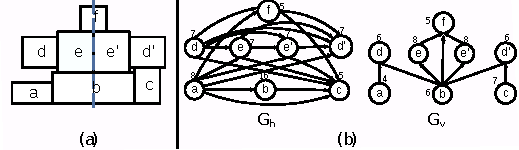
\includegraphics[height=0.17\textheight]{Figures/6.pdf}
  \caption{(a) Placement compact. (b) Représentation en {\it TCG} du placement compact (a).}
\label{fig:6}
\end{center}
\end{figure}

Les {\it Transitive Closure Graphs (TCG)} sont introduits par \cite{Lin2001} dans le contexte d'opter pour des solutions différentes des {\it sequence pairs} et des {\it B*-trees}. \cite{Zhang2008} y ajoute la considération des contraintes de symmétrie. Les {\it Transitive Closure Graphs TCG)} sont étendus au {\it TCG-S} par \cite{Lin2004a} et \cite{Ming2005} avec lesquels la phase de compactage est plus performante est inspiré de celle des {\it sequence pairs}.

\subsubsection{Sommaires des contraintes des représentations}
Au cours de ces deux dernières décennies, de nombreuses représentations topologiques ont été utilisées en couplage avec diverses contraintes. L'ensemble des articles mentionnés précédemment sont rassemblés dans le tableau récapitulatif \ref{tab:constraints}. A partir d'une représentation du plan de masse considérant les contraintes du concepteur, il en vient ensuite la phase d'optimisation du placement. Elle consiste à explorer l'espace des solutions de placement afin de trouver une solution en un temps raisonnable.
\begin{table}[h]
\footnotesize
\centering
\caption{Tableau récapitulatif de l'état de l'art des représentations de placement pour les circuits analogiques }
\label{tab:constraints}
  \begin{tabular}{|L{100pt}|C{50pt}|C{50pt}|C{50pt}|C{50pt}|C{50pt}|}
    \hline
    Contraintes                              & Slicing-tree                                                         & Sequence Pair & O-tree & B*-tree et HB*-tree & TCG \\ \hline
    Symmétries                                & \cite{Abthoff1996}, \cite{Prieto1997}, \cite{lina2012}, \cite{Wu2012}& \cite{Balasa2000}, \cite{Balasa2001}, \cite{Cheong2006}, \cite{Nakatake2010}, \cite{Xiao10}& \cite{FlorinBalasa2000}, \cite{LinfuXiao2009}& \cite{Balasa2000.2}, \cite{Balasa2002}, \cite{Maruvada2005}, \cite{Strasser08}, \cite{Lin09}, \cite{Lin2010}, \cite{Lin11}, \cite{Chou2011}, \cite{Tsao2011} &  \cite{Zhang2008}, \cite{Ming2005}   \\ \hline
    Symétrie de groupes                       & \cite{Wu2012}                                                        & \cite{Xiao10} & & \cite{Lin09}, \cite{Lin2010}, \cite{Lin11} &     \\ \hline
    Centrage géométrique                      &                                                                      & \cite{Xiao10} & \cite{LinfuXiao2009}& \cite{Strasser08}                    &     \\ \hline
    Sens du courant                           & \cite{Wu2012}                                                        & \cite{Long2006}&        &                    &     \\ \hline
    Température                               &                                                                      &                &        & \cite{Lin11}       &     \\ \hline
    Régularité                                &                                                                      &\cite{Nakatake2010}&        &  \cite{Chou2011}&     \\ \hline
    Proximité                                 & \cite{Abthoff1996}, \cite{Young2000}                                 &\cite{Cheong2006}&        & \cite{Strasser08} &     \\ \hline
    Régularité                                &                                                                      &               &        & \cite{Balasa2000.2} &     \\ \hline
    Modules pré-placés                        & \cite{Abthoff1996}, \cite{Young1998}                                 &               &        & \cite{Tsao2011}     &     \\ \hline
    Bordures                                  & \cite{Young1999}                                                     &               &        & \cite{Lin2010}, \cite{Tsao2011}      &     \\ \hline
    Routage                                   & \cite{Prieto1997}                                                    &\cite{Xiao10}  &        &                     &     \\ \hline
  \end{tabular}
\end{table} \newpage

\subsection{Les méthodes d'optimisation de placement}
\label{sec:Placement-SoA-optimization}
La majeure partie des approches de l'état de l'art utilise une représentation topologique parmi celles mentionnées dans la section précédente, avec laquelle on applique la méthode du recuit simulé. Cette méthode introduite par \cite{kirkpatrick83} est une technique probabiliste d'approximation de l'optimum global d'une fonction donnée. C'est à dire qu'il s'agit d'une métaheuristique permettant d'estimer l'optimisation globale dans un grand espace de recherche. Le principe s'inspire du processus de recuit des métaux en métallurgie dans lequel le refroidissement d'un matériau est contrôlé. Cela se traduit par une probabilité d'acceptation dégressive des mauvaises solutions dans l'espace de solutions exploré. \newline

Le fonctionnement de l'algorithme du recuit simulé se déroule par les étapes suivantes:
\begin{enumerate}
\item \label{enum:i1} L'algorithme sélectionne une transformation aléatoire prédéfinie sur la solution courante 
\item \label{enum:i2} On mesure la qualité de la solution sélectionnée 
\item On sauvegarde la nouvelle solution ou bien on décide maintenir la solution courante en se basant sur une probabilité dépendant de la qualité précédemment évaluée
\item Le paramètre de température diminue se traduisant par une augmentation de la probabilité du choix de la meilleure solution et une diminution de la probabilité du choix de mauvaise qualité
\end{enumerate}
Le tirage au sort (étape \ref{enum:i1}) des transformations est déterminé en fonction de l'approche choisie. Ces transformations dépendent de la représentation utilisée, une transformation revient à perturber le graphe représentant le placement de la solution courante. Il peut s'agir d'une rotation d'un module ou d'un échange de position entre deux modules. \newline 

La spécification des contraintes de placement d'un concepteur se définit par la formulation d'une fonction de coût qui nous permet d'évaluer la qualité (étape \ref{enum:i2}) de la solution sélectionnée . Afin d'illustrer le fonctionnement général d'une fonction de coût, considérons une optimisation sur une contrainte de surface global et d'une longueur de fil, la fonction de coût se présenterait de la façon suivante:
\begin{equation}\label{eq:1}
  Cost(F) =  \alpha . A_{normalis \acute{e}} + \beta . W_{normalis \acute{e}}
\end{equation}
avec $\alpha$ et $\beta$ étant des paramètres de réglages permettant d'influencer l'importance de la contrainte considérée, $A_{normalis \acute{e}}$ représentant la surface total occupée normalisée et $W_{normalis \acute{e}}$ la longueur de fil totale normalisée.
\newpage
\section{Implémentation}
\label{sec:Placement-Implémentation}
Parmi l'ensemble des méthodologies de placement analogique, la majorité d'entre elle présente une capacité à produire un placement tenant compte d'une ou plusieurs contraintes du concepteur. L'utilisation de métaheuristique permet de produire des résultats optimisés pour les contraintes considées dans la fonction de coût. Néanmoins, la complexité des contraintes des circuits analogiques et mixtes peuvent rendre difficile l'ajustement des paramètres de la fonction de coût. Dans la section suivante, nous présenterons l'approche pour laquelle nous avons opté ainsi que les raisons qui nous ont poussés à faire ces choix. Un exemple illustrera notre méthodologie et notre outil de placement.

\subsection{Notre approche de placement}
La phase de placement est une étape complexe dans la réalisation d'un circuit tant pour les circuits numériques qu'analogiques mais se différencie par leur problème. Dans le cadre des circuits numériques, le problème consiste à placer un grand nombre de cellules tout en minimisant la surface occupée et la longueur de fils des interconnections. En règle générale, la phase de placement est découplé de la phase de routage. Quant au problème de placement des circuits analogiques, il consite à placer un plus faible nombre de cellules tout en respectant les deux contraintes mentionnées précédemment, mais également une multitude de contraintes simultanément pouvant provenir de plusieurs domaines (électrique, mécanique ou bien thermique). \newline

Ces considérations ont amenées à la création de représentations topologiques et méthodes d'optimisation mentionnée dans les sous-sections \ref{sec:Placement-SoA-topologie} et \ref{sec:Placement-SoA-optimization}. En étudiant l'état de l'art du placement analogique, nous pensons que certains aspects nécessite une particulière attention ainsi que les limites d'une grande majorité des approches. Ce sont en tenant compte des considérations suivantes que nous avons effectué des choix dans le cadre de notre approche de placement:

\begin{itemize}
\item \textbf{Interventions du concepteur:} La conception du dessin des masques dans le domaine numérique est une étape particulièrement automatisé par rapport au domaine analogique. Du fait de la complexité du jeu de contraintes à gérer, nous jugeons qu'il est préférable de ne pas rendre l'automatisation du placement et du routage aussi automatique que dans le domaine numérique. Le placement d'un circuit dépend de plusieurs facteurs. L'environnement dans lequel va fonctionner le circuit comprend la prise en compte des effets des procédés de fabrication et des leurs effets parasites. Le facteur qui nous parait particulièrement important est que l'expérience d'un concepteur peut énormément influencer les choix de placement dans la gestion des compensations des effets parasites. Sans la prise en compte de cette experience, les outils de placement pour circuits analogiques produiront la plupart du temps des résultats insatisfaisant. Il en vient qu'il est nécessaire que le concepteur ait la possibilité des d'effectuer des interventions significatives. Notre approche s'oriente vers une approche o\`u l'automatisation est moindre en comparaison à l'état de l'art mais l'influence du concepteur sur le résultat final d'avantage prise en compte.

\item \textbf{Gestion des contraintes:} On observe dans l'état de l'art qu'une grande diversité de contraintes pour chaque représentation topologique en particulier pour les {\it B*-trees}. On remarque que la gestion des contraintes est relativement automatisé, il n'est pas toujours évident de connaître la capacité des paramètres à être modifier. L'ajustement de ces paramètres est généralement fixé suite à de nombreux essaies et ne peut être l'unique manoeuvre de jeu du concepteur. Dans notre méthodologie de placement, les contraintes gérées de manière automatique sont uniquement les contraintes de symétries. Nous utilisons une approche en {\it slicing tree}, cette représentation sera défini par le concepteur. Définir le {\it slicing tree} revient à laisser le choix aux concepteurs de juger l'importance de chacune des contraintes nécessaires à être prise en compte.

\item \textbf{Ajustabilité du placeur:} Le recuit simulé associé à une des représentations de l'état de l'art permet de générer des placements suivant en certains nombres de critères. Malgrés la qualité des placements produits, il est souvent nécessaire de réaliser des modifications diverses. Il peut s'agir de modification de placement entre deux blocks ou bien un simple repositionnement de certains modules. Dans la mesure o\`u les concepteurs souhaitent réaliser ce type de modifications, il peut s'avérer difficile de réajuster la représentation topologique ou bien encore la position de l'ensemble du circuit pour des raisons de compactions. Dans le cadre du {\it slicing tree}, le repositionnement ou bien le changement de taille d'un module est facile de part la structure du plan de masse en découpe. Tout comme mentioné dans le point précédent, la définition du {\it slicing tree} est une tâche réalisée par le concepteur, lui permettant d'avoir un contrôle important sur le placement relatif des modules.

\item \textbf{Placement déterministe:} Les algorithmes d'optimisation ne permettent pas toujours de générer des placements prévisibles. Certains d'entre eux permettent une certaine reproductibilité à maintenant les jeux de paramètres du recuit simulé en tenant compte de la température de départ et de la fonction de refroidissement. Néanmoins, les aspects aléatoires des probabilités des choix de placement peuvent rendre l'algorithme non déterministe. Le non-déterminisme rend l'évaluation des paramètres d'entrées difficiles ainsi que l'ajustabilité du placeur. L'approche que nous avons adopté permet un calcul des placements valides de manière déterministe. Nous jugeons que cette caractéristique est particulièrement utile dans les phases de débug.
\begin{figure}[h]
\begin{center}
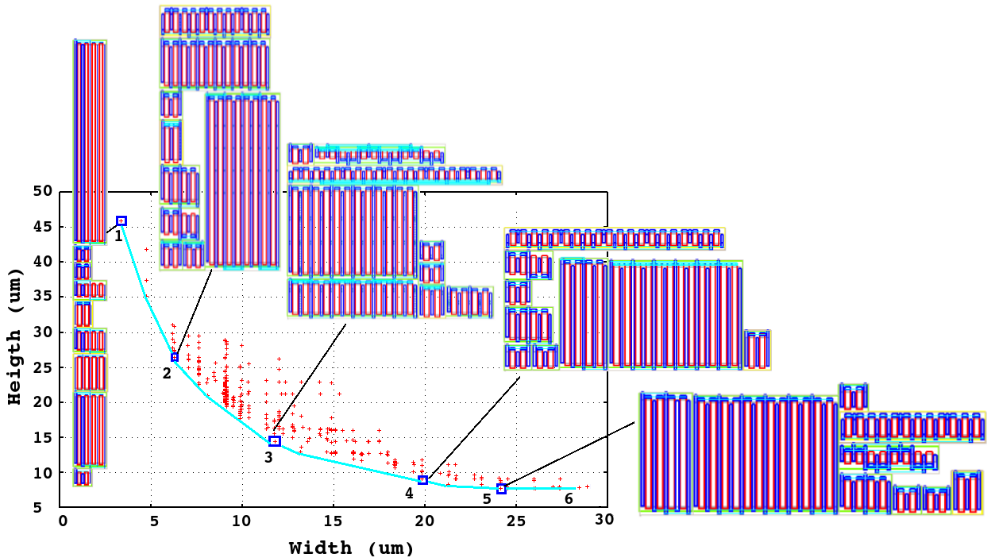
\includegraphics[height=0.25\textheight]{Figures/7-1.png}
\caption{Notre approche permet la génération rapide de plusieurs placements}
\label{fig:3}
\end{center}
\end{figure}
\item \textbf{Choix multiple de placements:} Le recuit simulé permet de générer un unique placement optimisé respectant au mieux les contraintes données considérées en entrée. Pour les même raisons mentionées dans les points précédents, cet unique placement sera probablement rarement choisi par tous les concepteurs. Nous pensons qu'il est nécessaire d'avoir la capacité à générer plusieurs placements afin que les concepteurs puissent choisir une solution qui lui conviennent. Certains placements peu compactes pourraient être des résultats de placements plus satisfaisant aux yeux des concepteurs dans certaines situations. Les placements identifiés par notre outil de placement sont disposés sur un graphe o\`u chaque placement est représenté par un point défini par la largeur et hauteur du placement global.

\item \textbf{Placement déterministe:} Les algorithmes d'optimisation ne permettent pas toujours de générer des placements prévisibles. Certains d'entre eux permettent une certaine reproductibilité à maintenant les jeux de paramètres du recuit simulé en tenant compte de la température de départ et de la fonction de refroidissement. Néanmoins, les aspects aléatoires des probabilités des choix de placement peuvent rendre l'algorithme non déterministe. Le non-déterminisme rend l'évaluation des paramètres d'entrées difficiles ainsi que l'ajustabilité du placeur. L'approche que nous avons adopté permet un calcul des placements valides de manière déterministe. Nous jugeons que cette caractéristique est particulièrement utile dans les phases de débug.


\begin{table}[h]
\footnotesize
\centering
\caption{Comparison of area usage and runtime for different approaches on 1-S symmetry placement  \cite{Xiao10}}
\label{tab:implémentation}
\begin{tabular}{|c|c|c|c|c|c|c|c|c|c|c|}
\hline
\multirow{2}{*}{Data Set} & \multirow{2}{*}{\begin{tabular}[c]{@{}c@{}}Block \\ No.\end{tabular}} & \multirow{2}{*}{\begin{tabular}[c]{@{}c@{}}1-D\\ Groups\end{tabular}} & \multicolumn{2}{c|}{Sequence Pair} & \multicolumn{2}{c|}{Slicing Tree} & \multicolumn{2}{c|}{HB*-tree} & \multicolumn{2}{c|}{B*-tree} \\ \cline{4-11} 
                          &                                                                       &                                                                       & Area        & Time      & Area        & Time      & Area           & Time         & Area          & Time         \\ \hline
Bench 1                   & 65                                                                    & 8,12,5                                                                & 114.9       & 780       & 114.9       & 246       & 104.7          & 22           & 104.9         & 337          \\ \hline
Bench 2                   & 110                                                                   & 16,6,6,12,4                                                           & 110.4       & 2824      & 109.4       & 726       & 105.7          & 43           & 107.7         & 387          \\ \hline
\end{tabular}
\end{table}

\item \textbf{Temps d'exécution faible:} Les contraintes de placement pour les circuits analogiques ainsi que le nombre inférieur de cellules réduit fortement l'espace de solutions en comparaison avec le problème du placement des circuits numériques. Le temps d'execution du recuit simulé nécessite un certain temps quelque ce soit le type de topologie employé \cite{Xiao10}. La génération de multiple placements de notre approche nécessite des temps de placements inférieurs à ceux de l'état de l'art. Le temps requis pour passer d'un placement à un autre est de l'ordre de l'intéractif.

\item \textbf{Considérations pour la phase de routage:} Le point le plus crucial dans la comparaison entre notre approche de placement et l'état de l'art. La majeure partie de l'état étudie le problème de placement des circuits analogiques ne manière découplé avec la phase de routage. Or la phase de routage ne peut être totalement ignorée dans la phase de placement. La situation concrête justifiant cela est qu'un placement peut être considéré placé de manière optimiser sur la base de critères de surface occupée. Un circuit trop congestioné ne laissera pas assez de place pour les fils de routage. Contrairement aux circuits numériques, certains fils de routage ne peuvent être tirés au-dessus de certains parties analogiques. \'Ecarter un circuit compacte deviendrait alors un travail extrêmement complexe et dénaturerait le résultat de placement initial. De part sa structure, le {\it slicing tree} n'est pas reconnu comme étant la représentation topologique la plus compacte mais elle est particulièrement flexible pour considérer des espaces dédiées aux fils de routage. En plus de la représentation topoligique, nos outils sont uniformes d'un point de vue logiciel. Les objets de manipuler lors de la phase de placement sont réutiliser dans le cadre du routage permettant évitant ainsi des pertes d'informations lors de conversion ou des problèmes couplages entre deux outils developpés distinctement.
\begin{figure}[t]
\begin{center}
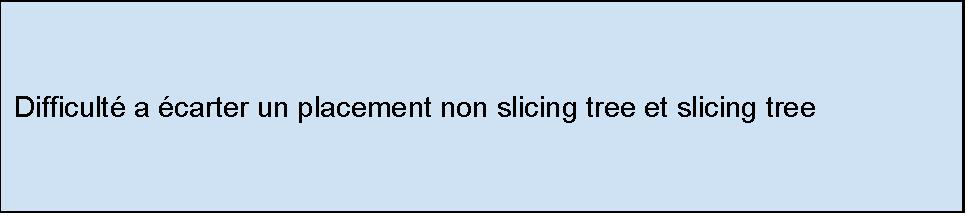
\includegraphics[height=0.10\textheight]{Figures/8.pdf}
\caption{Difficultés à écarter un placement non slicing-tree}
\label{fig:8}
\end{center}
\end{figure}
\end{itemize}
\subsection{Méthodologie de placement}
Notre méthodologie de placement consiste à effectuer un placement automatisé tout en impliquant des prises de décisions des concepteurs. L'objectif est de permettre à chaque concepteur de pouvoir appliquer ses propres contraintes sans engendrer une automatisation trop avancée. Cela entrainera des résultats moins optimisés en termes de surface mais en contre partie, le placement seront plus prévisibles et plus simplement ajustables. L'organisation de notre méthodologie se présente de la manière suivante:
\begin{itemize}
\item \textbf {La topologie en \textit{slicing tree}:} le concepteur définit une position relative des modules.
\item \textbf {Expression des contraintes de placement:} le concepteur introduit un ensemble de contraintes de placement.
\item \textbf {Algorithme de placement:} l'outil établit les placements possibles et génère un placement choisi par le concepteur.
\end{itemize}
\label{sec:Placement-methodologie}

\subsubsection{Définition d'une topologie de placement}
Lors de la conception d'un système sur puce (SoC), les espaces dédiés aux circuits numériques et analogiques sont distincts afin que chacun des circuits puissent être conçus de manière indépendante en terme de surface de circuit. Les circuits numériques sont connus pour leur structure regulière en bande dans lesquelles les cellules standards sont placées et routées sachant leurs connectivités. C'est avec cette idée de bandes que de nombreux circuits analogiques sont également organisés. Pour les circuits analogiques, ces bandes sont en revanche hétérogènes et dépendent de la hauteur des modules qui les constituent. Ces bandes ne s'étendent pas d'une extrémité à une autre du circuit mais se limitent à un groupe de modules soumis à des contraintes de proximités dû à leurs connectivités. Placer les modules de cette façon permet d'obtenir des circuits réguliers ce qui est un aspect critique pour certains circuits analogiques qui nécessitent d'évoluer dans un environnement le plus semblable possible. \newline

Avec l'objectif de représenter l'organisation en bande, nous avons opté pour le choix de la représentation des \textit{slicing trees}. Mentionné dans la section \ref{sec:Placement-SoA-topologie}, un \textit{slicing tree} est une représentation topologique qui consiste à définir un espace divisé par de nombreuses fois verticalement ou horizontalement. Ces divisions d'espace forment alors un ensemble de régions rectangulaires qui chacun peut représenter un module ou bien un espace vide pouvant être utilisé pour la phase de routage. Ces divisions sont organisées de manière hiérarchique et forment un graphe dans lequel chaque noeud hiérarchique est soit une division verticale, soit une division horizontale. Il en revient aux concepteurs la tâche de définir un \textit{slicing tree} et sa définition du \textit{slicing tree} ne sera pas altérée par notre outil de placement. Les seuls perturbations subies seront les écartements de modules afin d'y faire passer les fils de routage. En définissant eux-même la représentation topologique, les concepteurs seront libre de jugé par eux-même l'importance des contraintes de proximité, régularité ou de bordudes en fonction de l'environnement dans lequel se trouve le circuit et leurs expériences personnelles en tant que concepteur.\newline
\begin{figure}[h]
\begin{center}
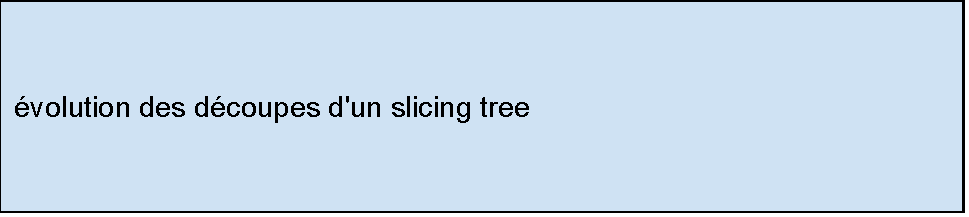
\includegraphics[height=0.10\textheight]{Figures/9.pdf}
\caption{Difficultés à écarter un placement non slicing-tree}
\label{fig:9}
\end{center}
\end{figure}\newline
\indent Fig. \ref{fig:9} présente une construction de graphe de \textit{slicing trees} pour un placement donné. On peut y observer les découpes hiéarchiques horizontales et verticales. La représentation en \textit{slicing trees} ne permet pas de représenter tous les placements possibles et un exemple de placement non représentable est donné par la figure \ref{fig:10}. Dans une certaine mesure, il est possible de représenter ces placements avec un \textit{slicing tree} mais la compaction et la surface du circuit occupées seront dégradées. Cependant, nous jugeons qu'il est plus important de prendre en compte la faisabilité du circuit en tenant compte de la capacité à espacer les modules d'un placement donné. La représentation en \textit{slicing tree} est adaptée à ces écartements, on considère que chaque découpe vertical ou horizontal puisse être un espace de routage qu'on agrandit en largeur pour une découpe verticale et en hauteur pour une découpe horizontale. \newline
\begin{figure}[h]
\begin{center}
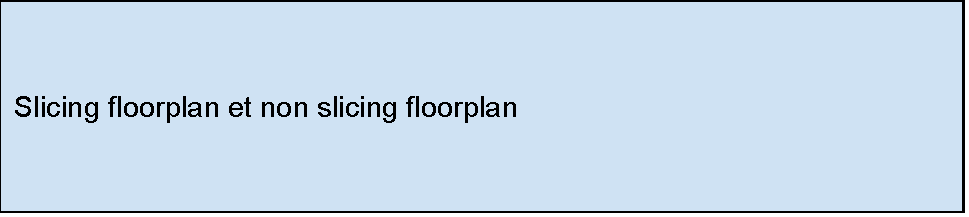
\includegraphics[height=0.10\textheight]{Figures/10.pdf}
\caption{(a) Placement représentable par un \textit{slicing tree} (b) Placement non représentable par un \textit{slicing tree}}
\label{fig:10}
\end{center}
\end{figure} 
\subsubsection{Expression des contraintes de placement}
On décompose les éléments d'un \textit{slicing trees} de la façon suivante:
\begin{itemize}
\item \textbf{les devices}
\item \textbf{les espaces de routage}
\item \textbf{Les rails traversant}
\item \textbf{les noeuds hiérarchiques}
\end{itemize}

On définit un device comme étant un bloc numérique ou analogique. Dans le cadre d'un bloc analogique, il peut s'agir d'une cellule numérique contenant une ou plusieurs cellules standards. Pour un bloc analogique, un device peut représenter un ensemble de transistors permettant de réaliser une fonction analogique de base. Ces devices peuvent être un simple \textbf{transistor}, une \textbf{paire différentielle}, un \textbf{miroir de courant}, un \textbf{montage en cascode} ou un \textbf{cross-coupled pair}. La raison pour laquelle ces blocs ont été définie est que le comportement électrique de ces blocs analogiques nécessite un dessins des masques dédié comprenant des contraintes géométriques fortes liées au placement et au routage. Ils peuvent également être générés selon des styles dessins des masques tels quepar centrage géométrique ou de manière interdigité. Ces blocs analogiques sont générés de manière correcte par construction à partir des règles de dessins de la technologie donnée. De plus, chacun des devices est paramétrable et contient les estimations des parasites liés à son dessin des masques. Pour plus de détails concernant notre librarie de devices analogiques, \cite{youssef2012} décrit entièrement le contenu de ces devices.

Dans le contexte du \textbf{slicing tree}, un device est défini par plusieurs attributs:
\begin{itemize}
\item \textbf{Une coordonnée x, y}: Elle représente la position du coin inférieur gauche du device au sien du plan considéré pour le placement des devices.
\item \textbf{Une hauteur et une largeur}: Elle définit le rectangle englobant la surface occupée par le device.
\item \textbf{Une contrainte d'alignement}: Elle positionne le device au sein du noeud hiéarchique, d'avantage de détails seront donnés dans la description d'un noeud hiéarchique. 
\item \textbf{Variation du nombre de doigts des transistors}: Les configurations en nombre de doigts de transistors tolérées par le concepteur.
\end{itemize}

\begin{figure}[h]
\begin{center}
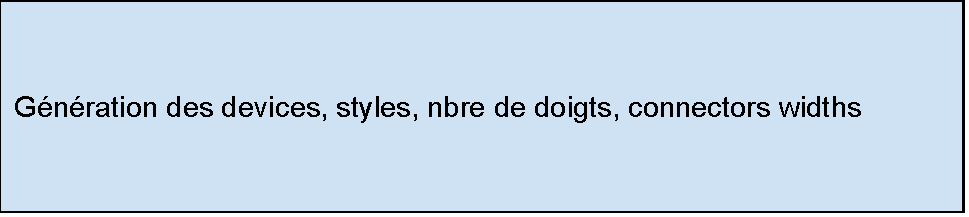
\includegraphics[height=0.11\textheight]{Figures/12.pdf}
\caption{Les paramètres réglables des devices, (a) Style de dessin des masques, (b) Variation du nombre de doigts et (c) Variation de la taille des connecteurs.}
\label{fig:12}
\end{center}
\end{figure} 
Notre approche de placement consiste à organiser les devices en bande et on cherche également à faire sorte que les devices d'une bande possèdent une hauteur le plus similaire possible. Afin d'obtenir cette configuration, il est nécessaire de considérer plusieurs aspect ratios pour chacun des devices en faisant varier le nombre des doigts des transistors des blocs analogiques tout en préservant leur fonctionalité électrique. Néanmoins, nous sommes conscient que cette action implique une variation de la capacité source/drain $C_{jSB}$ pouvant influencer les performances du circuits. \cite{Long2006} et \cite{Wu2014} détaille cette influence de la variation du nombre de doigts d'un transitor. Cependant, dans le cadre de notre approche, notre objectif consiste à effectuer plusieurs boucles itératives sur l'ensemble du design et ainsi resserrer les contraintes du circuit à chaque nouvelle itération afin de tendre vers une solution souhaitée. \newline
 
\indent Les espaces de routage sont des espaces vides dédiés au positionnement des fils de routage. Au sein d'un \textbf{slicing tree}, chaque découpe du circuit est considéré comme un espace de routage rectangulaire redimensionnable dans une seule direction. Dans le cas d'une découpé verticale, l'espace de routage peut être redimensionné de manière horizontale et on appelle ces espaces comme étant des espaces de routage verticaux. Réciproquement pour les découpes horizontales, l'espace de routage peut être redimensionné manière verticale et on appelle ces espaces comme étant des espace de routage horizontaux. Les espace de routage représentant une découpe du \textbf{slicing tree} sont implicites et ne nécessitent pas d'être précisé par l'utilisateur. Pour des raisons de clareté, les espaces de routage dûs à une découpe du \textbf{slicing tree} ne seront pas représentés sur un \textbf{slicing tree}. En revanche, il est possible de considérer des espaces vides volontaires rectangulaires, ces derniers peuvent être utilisés pour des ajustements de position.\newline

\indent Dans le contexte du \textbf{slicing tree}, un espace de routage est défini par plusieurs attributs:
\begin{itemize}
\item \textbf{Une coordonnée x, y}: Elle représente la position doi inférieur gauche de l'espace de routage au sien du plan considéré.
\item \textbf{Une hauteur ou une largeur}: Elle définit l'épaisseur de la découpe (largeur pour une découpe verticale et hauteur pour une découpe horizontale).
\end{itemize}
\begin{figure}[h]
\begin{center}
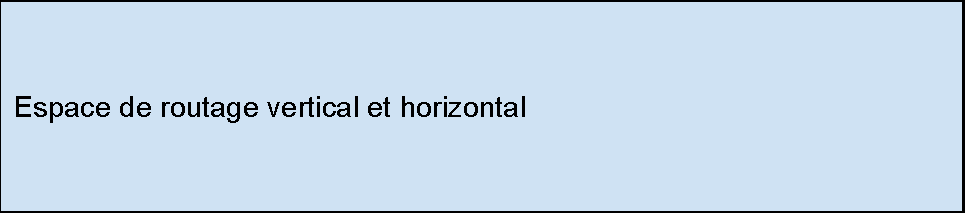
\includegraphics[height=0.11\textheight]{Figures/13.pdf}
\caption{Espace de routage vertical et horizontal}
\label{fig:12}
\end{center}
\end{figure} 

Les noeuds hierarchiques représentent les découpes hierarchiques verticales et horizontales du circuit. Ces noeuds permet la gestion des contraintes appliqués aux devices tels que les contraintes d'alignement et gèrent également les contraintes de symétries des devices. Chaque noeud hiéarchique possède des noeuds fils pouvant être des devices, des espaces de routage, des rails ou un autre noeud hierarchique et gère la propagation des contraintes soumis par le concepteur vers les racines du \textbf{slicing tree} ainsi qu'aux espaces de routage implicites dûs aux découpes. Les noeuds hierachiques propagent également les aspects ratios des devices en \textbf{bottom-up} jusqu'à la racine du \textbf{slicing tree} qui représente les aspects ratios globales du circuit. \newline

\indent Dans le contexte du \textbf{slicing tree}, un noeud hiéarchique est défini par plusieurs attributs:

\begin{itemize}
\item \textbf{Une coordonnée x, y}: Elle représente la position du coin inférieur gauche de l'espace occupé par le noeud hiéarchique et ses noeuds fils.
\item \textbf{Une hauteur et une largeur}: Elle définit le rectangle englobant la surface occupée par l'espace occupé par le noeud hiéarchique et ses noeuds fils.
\item \textbf{Une contrainte d'alignement}: Elle positionne le noeud hiérarchique au sein du noeud hiéarchique supérieur.
\item \textbf{Ensemble de noeuds fils}: L'ensemble des noeuds fils est stocké dans un ordre déterminé déterminant le positionnement.
\item \textbf{Les symmétries}: Les noeuds fils symétriques sont stockés au niveau du noeud parent.
\item \textbf{Paramètre de validité}: La différence de taille entre device est souvent importante. Afin de se rapprocher le plus possible d'une topologie en bande, ce paramètre permet de spécifier la différence de taille autorisé pour considérer la bande comme étant un placement valide.
\end{itemize}
\begin{figure}[h]
\begin{center}
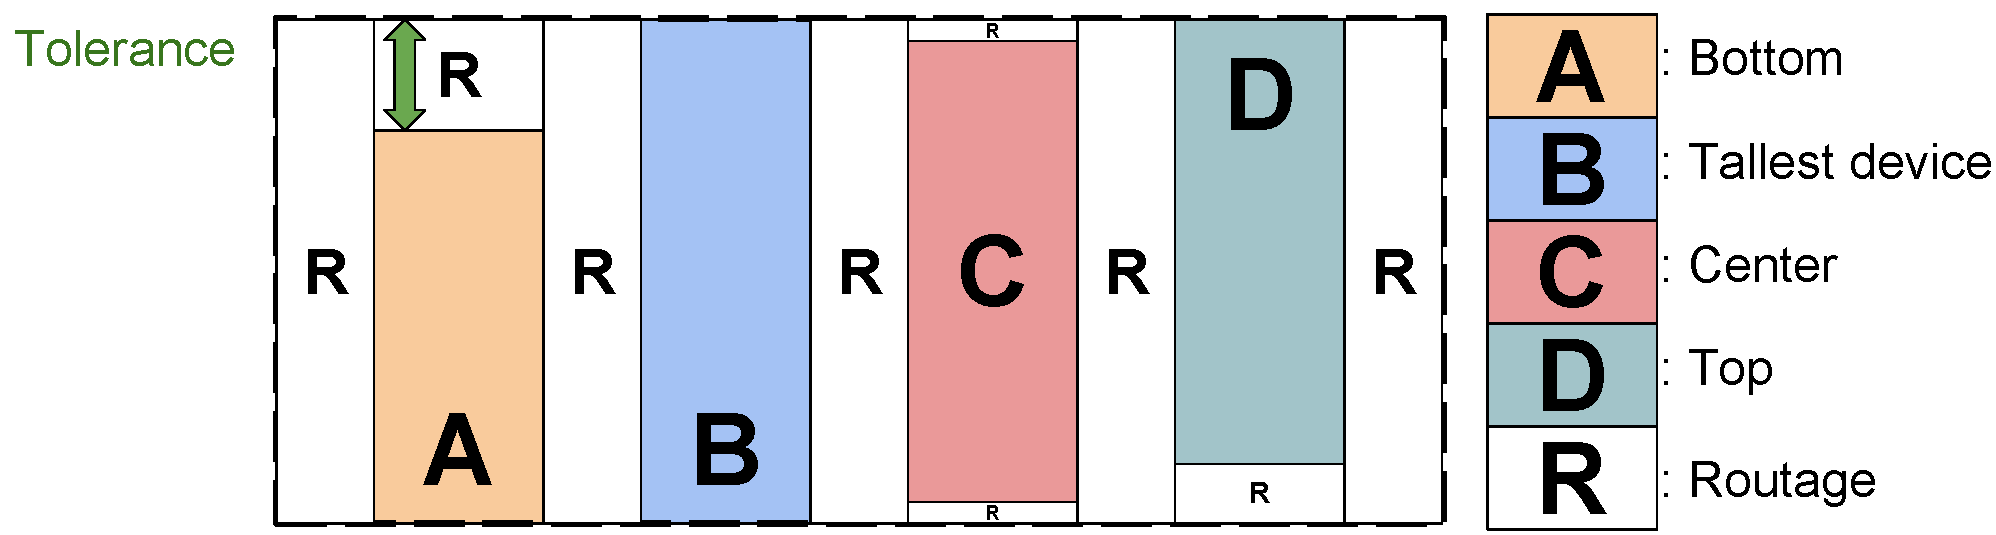
\includegraphics[height=0.15\textheight]{Figures/14.pdf}
\caption{Noeud hiérarchique vertical avec une organisation en bande}
\label{fig:14}
\end{center}
\end{figure} 

La figure \ref{fig:14} présente l'organisation d'un noeud hiérachique vertical. On y observe l'organisation d'une bande dans laquelle les devices $A$, $B$, $C$ et $D$ sont soumis à des contraintes d'alignement. La hauteur et la largeur d'un noeud hiérarchique vertical est déterminé par la formule suivante:
\begin{equation}
\begin{aligned}
Largeur_{BandeVerticale} &= \sum_{i=0}^{n} L_{NoeudFils_i} + \sum_{j=0}^{n+1} L_{EspaceDeRoutage_j} \\
Hauteur_{BandeVerticale} &= Max\{H_{NoeudFils_0},H_{NoeudFils_1}, ... , H_{NoeudFils_n}\}
\end{aligned}
\end{equation}
en considérant $n$ le nombre total de noeuds fils. Chaque espace noté "$R$" représente un espace de routage et sont dû soit à une découpe verticale soit à une différence de taille avec le noeud fils ayant la plus grande hauteur qui est "$B$" dans le cas ci-dessus. La taille d'un espace de routage dépend du nombre de fils de routage verticaux et de leur positinnement au sein de l'espace, d'avantage de détails seront donnés dans le chapitre sur le routage. Concernant les contraintes d'alignement à chacun des devices, "$A$" est aligné vers le bas de la bande, "$C$" est centré par rapport à la hauteur de la bande et "$D$" est aligné vers le haut de la bande. Les symétries au sein d'un noeud hierarchique se traduisent par la garantie que deux fils d'un noeud fils soient de la même taille et possède le même alignement. Sur la figure \ref{fig:14}, la boite englobante en pointillé représente l'espace du noeud hiéarchique considéré par les noeuds hiearchiques supérieurs.


\begin{figure}[h]
\begin{center}
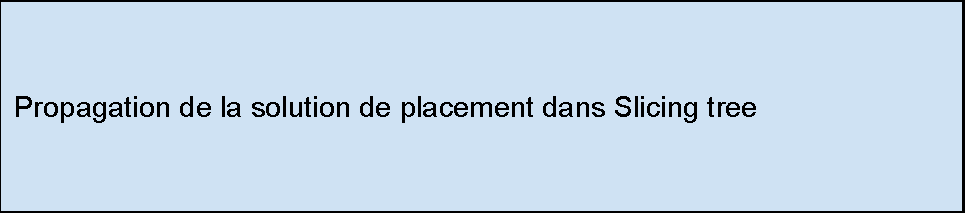
\includegraphics[height=0.11\textheight]{Figures/15.pdf}
\caption{Propagation des dimensions du placement dans un \textbf{slicing tree}}
\label{fig:11}
\end{center}
\end{figure} 

\begin{figure}[h]
\begin{center}
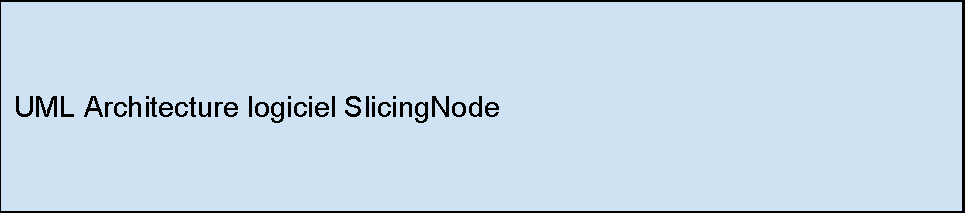
\includegraphics[height=0.11\textheight]{Figures/11.pdf}
\caption{Interface de programmation du placeur analogique et mixte}
\label{fig:11}
\end{center}
\end{figure} 
- API SlicingTree: Architecture logiciel ~1 page
- SlicingNode: 
DSlicingNode: NodeSets (number of fingers, dimensions), definition of what we call device? Layout style?
RoutingNode : Width of the channel, variable length depending on vertical or horizontal nodes
HSlicingNode et VSlicingNode: containing DSlicingNode, modificateur/accesseur (add, remove, find)
get Width/Height
slicing routing
adjust border slicing routing

Symmétries:
- symmetries inside a same level of hierarchie
- 2 blocks can be set to have the same dimensions

\subsubsection{Algorithme de placement}

How
- variation devices, layout styles
- Margin tolerances: Imposer des contraintes afin de limiter le nombre de placement possible
- Algorithme de calcul du nombre de placement possibles + Execution HVState ?
- Placement + stored placement

\section{Exemples}
\label{sec:Placement-Exemple}
What
- gmchamla
- Expliquer la structure de la description python
- Etapes à suivre avec l'execution des outils + screen des étapes
- Interface graphique, choix des positions et parametres de selections
- Différents résultats de placement à montrer
\section{Conclusion}